\section{Expected Outcomes}
\begin{enumerate}
\item A functional motor health monitoring device will be developed and tested.
\item The predictive maintenance algorithm will be formulated and proved from a selection
of diverse methods.
\item The controller supporting circuitry will be developed with a custom printed circuit
board.
\item nathan mutuma Electric motor system performance and efficiency will be optimized using insights from real-time data collected.
\end{enumerate}
\newpage
\section{Project Budget}
\setlength{\arrayrulewidth}{0.5mm}
\setlength{\tabcolsep}{18pt}
\renewcommand{\arraystretch}{1.5}
	\begin{tabular}{ |p{3cm}|p{3cm}|p{3cm}|p{3cm}|  }
		\hline
		\multicolumn{4}{|c|}{\textbf{Item List}} \\
		\hline
		ITEM & SPECIFICATION & QUANTITY & PRICE \\
		\hline
		Arduino & Uno Rev3, usb 2.0 Cable Type A/B & 1 & 3000 \\
		\hline
		Thermocouple Amplifier & MAX31855K & 1 & 1600 \\
		\hline
		WiFi Development Board & NodeMCU 32S ESP32/ CH340c  & 1 & 1400 \\
		\hline
		Thermocouple K type&Temp range: 0-600  & 1 & 1760\\
		\hline
		Thermocouple DH22 & 3.3-6v input  & 1 &750 \\
		\hline
		Power Unit & 12v/5W SMPS Module & 1   & 600\\
		\hline
		Breadboard & MB102  165*55*50mm & 2 & 400 \\
		\hline
		Jumper Wires & 20cm male 20cm female & 80 & 400 \\
		\hline
		\textbf{Total} & & &9910 \\
		\hline
	\end{tabular}

\section{Work Plan}
\begin{table}[!h]
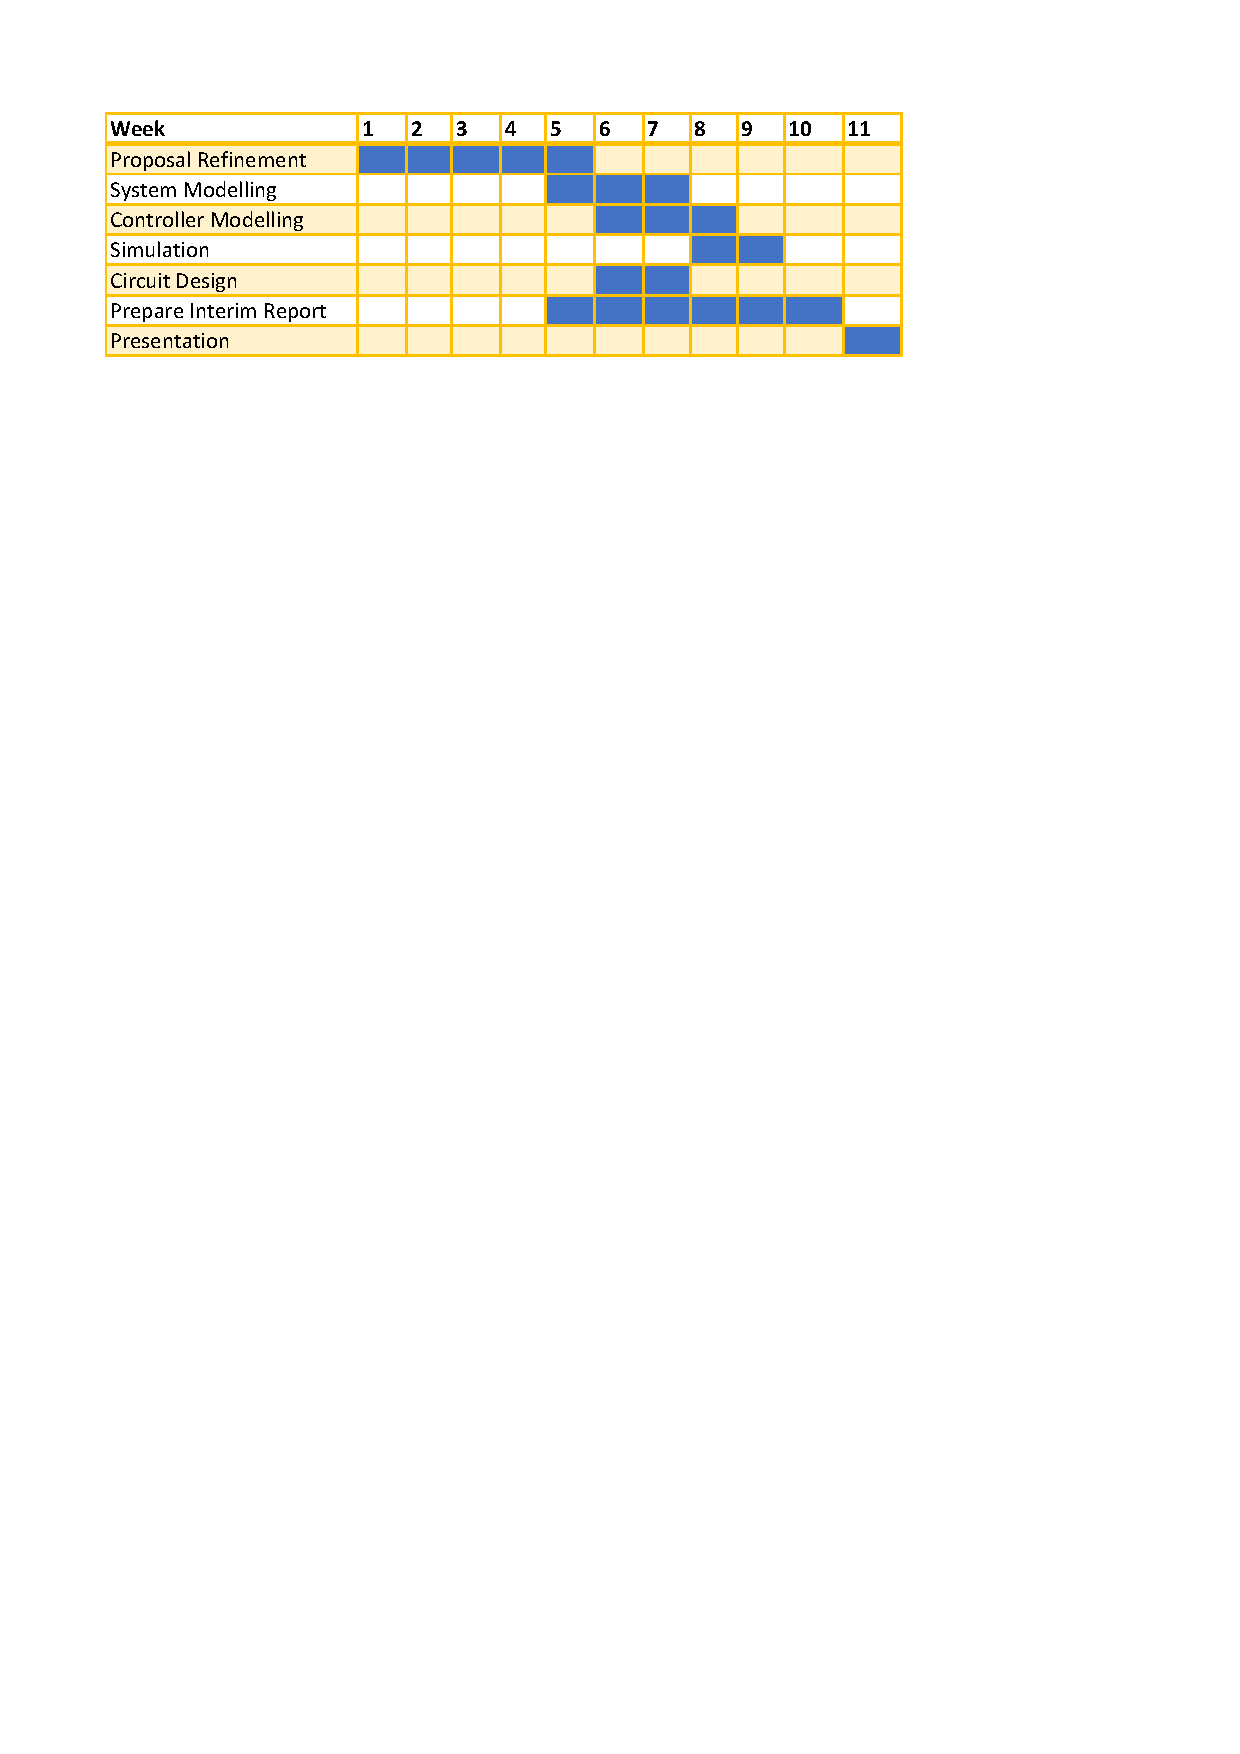
\includegraphics{Figures/workplan}
\caption{Workplan table}
\end{table}
